\section{Post-hoc Corpus-Size Diagnostic}
\paragraph{Post-hoc corpus-size diagnostic.}
The heterogeneous discovery gains are larger on tasks with larger evaluation corpora. Across 14 tasks, final $\Delta$ nDCG@10 versus $\log_{10}$ corpus rows has Spearman $\rho=0.587$ for Muon (200,000-permutation $p=0.030$) and $\rho=0.574$ for NorMuon ($p=0.035$). Both optimizers are positive on all seven larger-corpus tasks, compared with 3/7 and 4/7 on the smaller half. The association emerges mainly late and strengthens after excluding NQ. This analysis was designed after the association was visible, uses same-suite-selected discovery rates, and cannot distinguish corpus size from correlated task properties; we report it only as a clue motivating the independently frozen candidate-breadth diagnostic (Figure~\ref{fig:corpus-size-diagnostic}).

\begin{figure}[t]
\centering
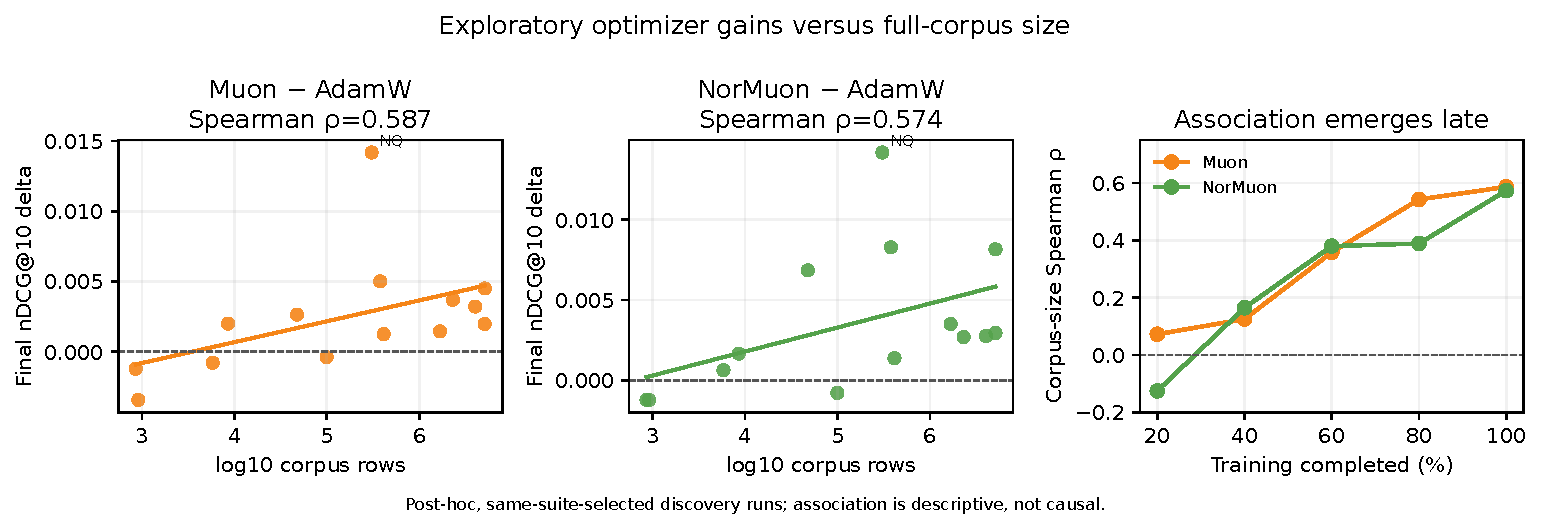
\includegraphics[width=\columnwidth]{../reports/corpus-size-diagnostic/corpus_size_association.pdf}
\caption{Post-hoc association between Muon-family discovery gains and full-corpus size. The right panel shows the association emerging across training stages.}
\label{fig:corpus-size-diagnostic}
\end{figure}
